\chapter{Nematoda and Arthropoda}\label{nematoda-and-arthropoda}

\section{Nematodes}\label{nematodes}

The \href{https://en.wikipedia.org/wiki/Nematode}{nematodes} or
roundworms constitute the phylum Nematoda (also called Nemathelminthes).
They are a diverse animal phylum inhabiting a broad range of
environments. Nematode species can be difficult to distinguish, and
although over 25,000 have been described, of which more than half are
parasitic, it is estimated that over 40,000 species exist. Nematodes are
classified along with insects and other moulting animals in the clade
Ecdysozoa, and, unlike flatworms, have tubular digestive systems with
openings at both ends. A characteristic of Nematoda is the one-way
digestive tract, with a pseudocoelom (body cavity made up of only an
ectoderm and endoderm).

Nematodes have successfully adapted to nearly every ecosystem from
marine (salt water) to fresh water, to soils, and from the polar regions
to the tropics, as well as the highest to the lowest of elevations. They
are ubiquitous in freshwater, marine, and terrestrial environments,
where they often outnumber other animals in both individual and species
counts, and are found in locations as diverse as mountains, deserts and
oceanic trenches. They are found in every part of the earth's
lithosphere, even at great depths, 0.9--3.6 km, below the surface of the
Earth in gold mines in South Africa. They represent 90\% of all animals
on the ocean floor. Their numerical dominance, often exceeding a million
individuals per square meter and accounting for about 80\% of all
individual animals on earth, their diversity of life cycles, and their
presence at various trophic levels point at an important role in many
ecosystems. The many parasitic forms include pathogens in most plants
and animals. A third of the genera occur as parasites of vertebrates;
about 35 nematode species occur in humans.

Nematodes are small, slender worms: typically approximately 5 to 100 µm
thick, and 0.1 to 2.5 mm long. The smallest nematodes are microscopic,
while free-living species can reach as much as 5 cm, and some parasitic
species are larger still, reaching over 1 m in length. The body is often
ornamented with ridges, rings, bristles, or other distinctive
structures.

The head of a nematode is relatively distinct. Whereas the rest of the
body is bilaterally symmetrical, the head is radially symmetrical, with
sensory bristles and, in many cases, solid `head-shields' radiating
outwards around the mouth. The mouth has either three or six lips, which
often bear a series of teeth on their inner edges. An adhesive `caudal
gland' is often found at the tip of the tail.

The epidermis is either a syncytium or a single layer of cells, and is
covered by a thick collagenous cuticle. The cuticle is often of complex
structure, and may have two or three distinct layers. Underneath the
epidermis lies a layer of longitudinal muscle cells. The relatively
rigid cuticle works with the muscles to create a hydroskeleton as
nematodes lack circumferential muscles. Projections run from the inner
surface of muscle cells towards the nerve cords; this is a unique
arrangement in the animal kingdom, in which nerve cells normally extend
fibres into the muscles rather than vice versa.

The oral cavity is lined with cuticle, which is often strengthened with
ridges or other structures, and, especially in carnivorous species, may
bear a number of teeth. The mouth often includes a sharp stylet, which
the animal can thrust into its prey. In some species, the stylet is
hollow, and can be used to suck liquids from plants or animals. The oral
cavity opens into a muscular, sucking pharynx, also lined with cuticle.
Digestive glands are found in this region of the gut, producing enzymes
that start to break down the food. In stylet-bearing species, these may
even be injected into the prey. There is no stomach, with the pharynx
connecting directly to a intestine (not surrounded by smooth muscle)
that forms the main length of the gut. This produces further enzymes,
and also absorbs nutrients through its single cell thick lining. The
last portion of the intestine is lined by cuticle, forming a rectum,
which expels waste through the anus just below and in front of the tip
of the tail. Movement of food through the digestive system is the result
of body movements of the worm. The intestine has valves or sphincters at
either end to help control the movement of food through the body.

Nitrogenous waste is excreted in the form of ammonia through the body
wall, and is not associated with any specific organs. However, the
structures for excreting salt to maintain osmoregulation are typically
more complex. In many marine nematodes, one or two unicellular `renette
glands' excrete salt through a pore on the underside of the animal,
close to the pharynx. In most other nematodes, these specialized cells
have been replaced by an organ consisting of two parallel ducts
connected by a single transverse duct. This transverse duct opens into a
common canal that runs to the excretory pore.

Four peripheral nerves run the length of the body on the dorsal,
ventral, and lateral surfaces. Each nerve lies within a cord of
connective tissue lying beneath the cuticle and between the muscle
cells. The ventral nerve is the largest, and has a double structure
forward of the excretory pore. The dorsal nerve is responsible for motor
control, while the lateral nerves are sensory, and the ventral combines
both functions. The nervous system is also the only place in the
nematode body that contains cilia, which are all non-motile and with a
sensory function. At the anterior end of the animal, the nerves branch
from a dense, circular nerve (nerve ring) round surrounding the pharynx,
and serving as the brain. Smaller nerves run forward from the ring to
supply the sensory organs of the head. The bodies of nematodes are
covered in numerous sensory bristles and papillae that together provide
a sense of touch. Behind the sensory bristles on the head lie two small
pits, or `amphids'. These are well supplied with nerve cells, and are
probably chemoreception organs. A few aquatic nematodes possess what
appear to be pigmented eye-spots, but is unclear whether or not these
are actually sensory in nature.

Most nematode species are dioecious, with separate male and female
individuals, though some, such as
\href{https://en.wikipedia.org/wiki/Caenorhabditis_elegans}{\emph{Caenorhabditis
elegans}}, are androdioecious, consisting of hermaphrodites and rare
males. Both sexes possess one or two tubular gonads. In males, the sperm
are produced at the end of the gonad and migrate along its length as
they mature. The testis opens into a relatively wide seminal vesicle and
then during intercourse into a glandular and muscular ejaculatory duct
associated with the vas deferens and cloaca. In females, the ovaries
each open into an oviduct (in hermaphrodites, the eggs enter a
spermatheca first) and then a glandular uterus. The uteri both open into
a common vulva/ vagina, usually located in the middle of the
morphologically ventral surface.

Reproduction is usually sexual, though hermaphrodites are capable of
self-fertilization. Males are usually smaller than females/
hermaphrodites (often much smaller) and often have a characteristically
bent or fan-shaped tail. During copulation, one or more chitinized
spicules move out of the cloaca and are inserted into the genital pore
of the female. Amoeboid sperm crawl along the spicule into the female
worm.

Eggs may be embryonated (containing an embryo) or unembryonated when
passed by the female, meaning their fertilized eggs may not yet be
developed. A few species are known to be ovoviviparous. The eggs are
protected by an outer shell, secreted by the uterus. In free-living
roundworms, the eggs hatch into larvae, which appear essentially
identical to the adults, except for an underdeveloped reproductive
system; in parasitic roundworms, the life cycle is often much more
complicated.

Nematodes as a whole possess a wide range of modes of reproduction. Some
nematodes, such as Heterorhabditis spp., undergo a process called
endotokia matricida: intrauterine birth causing maternal death. Some
nematodes are hermaphroditic, and keep their self-fertilized eggs inside
the uterus until they hatch. The juvenile nematodes will then ingest the
parent nematode. This process is significantly promoted in environments
with a low food supply.

Nematodes commonly parasitic on humans include ascarids
(\emph{Ascaris}), filarias, hookworms, pinworms (\emph{Enterobius}), and
whipworms (\emph{Trichuris trichiura}). The species
\href{https://en.wikipedia.org/wiki/Trichinella_spiralis}{\emph{Trichinella
spiralis}}, commonly known as the `trichina worm', occurs in rats, pigs,
and humans, and is responsible for the disease trichinosis.

\section{\texorpdfstring{\emph{Ascaris}}{Ascaris}}\label{ascaris}

\href{https://en.wikipedia.org/wiki/Ascaris}{\emph{Ascaris}} is a genus
of parasitic nematode worms known as the ``small intestinal
roundworms''. One species, Ascaris lumbricoides, affects humans and
causes the disease ascariasis. Their eggs are deposited in feces and
soil. Plants with the eggs on them infect any or ganism that consumes
them. A. lumbricoides is the largest intestinal roundworm and is the
most common helminth infection of humans worldwide. Infestation can
cause morbidity by compromising nutritional status, affecting cognitive
processes, inducing tissue reactions such as granuloma to larval stages,
and by causing intestinal obstruction, which can be fatal. The body is
long, cylindrical, fusiform (pointed at both the ends), body wall is
composed of cuticle, epidermis and musculature. Presence of a false body
pseudocoelom not lined by epithelium. Digestive system is complete.
Respiration by simple diffusion. Nervous system consists of a nerve ring
and many longitudinal nerve cords. Only sexual reproduction. Sexes are
separate with sexual dimorphism. Males are usually shorter than females.

\section{\texorpdfstring{View Prepared Slides of
\emph{Ascaris}}{View Prepared Slides of Ascaris}}\label{view-prepared-slides-of-ascaris}

\begin{enumerate}
\def\labelenumi{\arabic{enumi}.}
\tightlist
\item
  Female \emph{Ascaris} x.s. (Figure \ref{fig:ascaris})

  \begin{itemize}
  \tightlist
  \item
    Identify: oviduct, pseudocoelom, intestine with lumen (GVC), uterus,
    eggs, ventral nerve cord, longitudinal muscles, cuticle, excretory
    canal
  \end{itemize}
\end{enumerate}



\begin{figure}

{\centering \includegraphics[width=0.7\linewidth]{./figures/nematoda/ascaris_female}

}

\caption{Female \emph{Ascaris}.}\label{fig:ascaris}
\end{figure}

\section{\texorpdfstring{\emph{Trichinella}}{Trichinella}}\label{trichinella}

\href{https://en.wikipedia.org/wiki/Trichinella}{\emph{Trichinella}} is
the genus of parasitic roundworms of the phylum Nematoda that cause
trichinosis (also known as trichinellosis). Members of this genus are
often called trichinella or trichina worms. The genus was first
recognised in a larval form in 1835. The L1 larvae live in a modified
skeletal muscle cell. The adult worms occupy a membrane-bound portion of
columnar epithelium, living as intracellular parasites. Infections with
this genus have been reported from more than 150 different naturally or
experimentally infected hosts. It has been shown to have a worldwide
distribution in domestic and/or sylvatic animals. Trichinella is known
as the smallest human nematode parasite, yet it is also the largest of
all intracellular parasites. Oral ingestion of larvae-contaminated
tissue is the usual route of infection. Cooking pork meat properly or by
freezing pork, Trichinella infection can be prevented. However, freezing
pork is not an effective method for killing larvae.

\section{View Prepared Slides of
Trichinella}\label{view-prepared-slides-of-trichinella}

\begin{enumerate}
\def\labelenumi{\arabic{enumi}.}
\tightlist
\item
  \emph{Trichinella} encysted in muscle (Figure \ref{fig:trichinella})

  \begin{itemize}
  \tightlist
  \item
    Identify: muscle, cyst, larva
  \end{itemize}
\end{enumerate}



\begin{figure}

{\centering \includegraphics[width=0.7\linewidth]{./figures/nematoda/trichinella_encysted}

}

\caption{\emph{Trichinella} encysted in muscle.}\label{fig:trichinella}
\end{figure}

\section{Vinegar eels}\label{vinegar-eels}

\href{https://en.wikipedia.org/wiki/Turbatrix_aceti}{\emph{Turbatrix
aceti}} (vinegar eels, vinegar nematode) are free-living nematodes that
feed on the microbial culture, called mother of vinegar used to create
vinegar, and may be found in unfiltered vinegar. Vinegar eels are often
given to fry (baby fish) as a live food, like microworms. Although they
are harmless and non-parasitic, leaving eels in vinegar is considered
objectionable in the United States and is not permitted in vinegar
destined for American consumers. Manufacturers normally filter and
pasteurize their product prior to bottling, destroying the live
bacterial and yeast culture that these nematodes require for sustenance.

\section{Arthropods}\label{arthropods}

\href{https://en.wikipedia.org/wiki/Arthropod}{Arthropods} (from
arthron, ``joint'' and pous, ``foot'') are invertebrate animals having
an exoskeleton (external skeleton), a segmented body, and paired jointed
appendages. Arthropods form the phylum Euarthropoda, which includes
insects, arachnids, myriapods, and crustaceans. Arthropods are
characterized by their jointed limbs and cuticle made of chitin, often
mineralized with calcium carbonate. The arthropod body plan consists of
segments, each with a pair of appendages. The rigid cuticle inhibits
growth, so arthropods replace it periodically by molting.

Their versatility has enabled them to become the most species-rich
members of all ecological guilds in most environments. They have over a
million described species, making up more than 80\% of all described
living animal species, some of which, unlike most animals, are very
successful in dry environments.

Arthropods range in size from the microscopic crustacean Stygotantulus
up to the Japanese spider crab. Arthropods' primary internal cavity is a
hemocoel, which accommodates their internal organs, and through which
their hemolymph -- analogue of blood -- circulates; they have open
circulatory systems. Like their exteriors, the internal organs of
arthropods are generally built of repeated segments. Their nervous
system is ``ladder-like'', with paired ventral nerve cords running
through all segments and forming paired ganglia in each segment.

Their heads are formed by fusion of varying numbers of segments, and
their brains are formed by fusion of the ganglia of these segments and
encircle the esophagus. The respiratory and excretory systems of
arthropods vary, depending as much on their environment as on the
subphylum to which they belong.

Their vision relies on various combinations of compound eyes and
pigment-pit ocelli: in most species, the ocelli can only detect the
direction from which light is coming, and the compound eyes are the main
source of information, but the main eyes of spiders are ocelli that can
form images and, in a few cases, can swivel to track prey. Arthropods
also have a wide range of chemical and mechanical sensors, mostly based
on modifications of the many setae (bristles) that project through their
cuticles. Arthropods' methods of reproduction and development are
diverse; all terrestrial species use internal fertilization, but this is
often by indirect transfer of the sperm via an appendage or the ground,
rather than by direct injection.

Aquatic species use either internal or external fertilization. Almost
all arthropods lay eggs, but scorpions give birth to live young after
the eggs have hatched inside the mother. Arthropod hatchlings vary from
miniature adults to grubs and caterpillars that lack jointed limbs and
eventually undergo a total metamorphosis to produce the adult form. The
level of maternal care for hatchlings varies from nonexistent to the
prolonged care provided by scorpions.

The evolutionary ancestry of arthropods dates back to the Cambrian
period. The group is generally regarded as monophyletic, and many
analyses support the placement of arthropods with cycloneuralians (or
their constituent clades) in a superphylum Ecdysozoa.

Arthropods contribute to the human food supply both directly as food,
and more importantly indirectly as pollinators of crops. Some species
are known to spread severe disease to humans, livestock, and crops.

Arthropods belong to the phylum Euarthropoda. The phylum is sometimes
called Arthropoda, but strictly this term denotes a (putative - see
Tactopoda) clade that also encompasses Phylum Onychophora.

The appendages of arthropods may be either biramous or uniramous. A
uniramous limb comprises a single series of segments attached
end-to-end. A biramous limb, however, branches into two, and each branch
consists of a series of segments attached end-to-end.

The phylum Euarthropoda is typically subdivided into five subphyla, of
which one is extinct:

\begin{itemize}
\tightlist
\item
  Trilobites are a group of formerly numerous marine animals that
  disappeared in the Permian--Triassic extinction event, though they
  were in decline prior to this killing blow, having been reduced to one
  order in the Late Devonian extinction.
\item
  Chelicerates include horseshoe crabs, spiders, mites, scorpions and
  related organisms. They are characterized by the presence of
  chelicerae, appendages just above / in front of the mouth. Chelicerae
  appear in scorpions and horseshoe crabs as tiny claws that they use in
  feeding, but those of spiders have developed as fangs that inject
  venom.
\item
  Myriapods comprise millipedes, centipedes, and their relatives and
  have many body segments, each segment bearing one or two pairs of legs
  (or in a few cases being legless). They are sometimes grouped with the
  hexapods.
\item
  Crustaceans are primarily aquatic (a notable exception being woodlice)
  and are characterized by having biramous appendages. They include
  lobsters, crabs, barnacles, crayfish, shrimp and many others.
\item
  Hexapods comprise insects and three small orders of insect-like
  animals with six thoracic legs. They are sometimes grouped with the
  myriapods, in a group called Uniramia, though genetic evidence tends
  to support a closer relationship between hexapods and crustaceans.
\end{itemize}

\section{Crayfish}\label{crayfish}

\href{https://en.wikipedia.org/wiki/Crayfish}{Crayfish}, also known as
crawfish, crawdads, freshwater lobsters, mountain lobsters, mudbugs or
yabbies, are freshwater crustaceans resembling small lobsters, to which
they are related. They breathe through feather-like gills. Some species
are found in brooks and streams where there is running fresh water,
while others thrive in swamps, ditches, and paddy fields. Crayfish feed
on animals and plants, either living or decomposing, and detritus. Its
body is made up of twenty body segments grouped into two main body
parts, the cephalothorax and the abdomen. Each segment may possess one
pair of appendages, although in various groups these may be reduced or
missing. On average, crayfish grow to 17.5 centimeters in length, but
some grow larger. Walking legs have a small claw at the end.

\section{Crayfish Dissection}\label{crayfish-dissection}

\begin{enumerate}
\def\labelenumi{\arabic{enumi}.}
\tightlist
\item
  Get a dissction pan, scissorc, forceps, and a pointer.
\item
  Get a cray fish.
\item
  Place a crayfish on its side in a dissection tray (Fig.
  \ref{fig:crayfish}.
\item
  Locate the cephalothorax and the abdomen. The carapace, a shield of
  chitin, covers the dorsal surface of the cephalothorax. On the
  carapace, observe an indentation, the cervical groove, that extends
  across the midregion and separates the head and thoracic regions. On
  the thoracic region, locate the prominent suture or indentation on the
  cephalothorax that defines a central area separate from the sides.
  Note the individual segments of the abdomen.
\item
  Turn the crayfish with its dorsal side upward.
\item
  Locate the rostrum, which is the pointed extension of the carapace at
  the head of the animal. Locate the two eyes at the end of stalks.
\item
  Locate the five pairs of appendages on the head region. First locate
  the antennules in the most anterior segment. Behind them observe the
  much longer pair of antennae.
\item
  Turn the crayfish around with its ventral side upward.
\item
  Locate the mouth. Observe the mandibles (jaws), behind the antennae.
\item
  Locate the two pairs of maxillae, which are the last appendages in the
  cephalic region.
\item
  On the thoracic portion of the cephalothorax, observe the three
  pointed maxillipeds.
\item
  On the abdomen, observe six distinct segments. Observe a pair of
  swimmerets on each of the first five segments.
\item
  On the last abdominal segment, observe a pair of pointed appendages
  modified into a pair of uropods. In the middle of the uropods, locate
  the triangular-shaped telson.
\item
  Determine the sex of your specimen. Males (Fig. \ref{fig:malecray}
  have hardened gonapods and hooks on the third pair of legs. Females
  (\ref{fig:femalecray} have an opening to a seminal receptacle between
  the fifth pair of legs.
\item
  Turn the crayfish around so that its dorsal side is upward.
\item
  Use one hand to hold the crayfish dorsal side up in the dissecting
  tray, use scissors to carefully cut through the back of the carapace
  along the dotted line shown in figure \ref{fig:dorsal} below. Cut
  along the indentations that separate the thoracic portion of the
  carapace into three regions. Start the cut at the posterior edges of
  the carapace, and extend it along both sides in the cephalic region.
\item
  Using the forceps, carefully and slowly lift away the carapace.
\item
  Place the crayfish on its side (head facing left). Using scissors, cut
  starting at the base along the dotted line shown in Figure
  \ref{fig:lateral}. Extend the cut line forward toward the rostrum (at
  the top of the head).
\item
  Use forceps to carefully lift away the remaining parts of the
  carapace, exposing the underlying gills and other organs.
\item
  Locate and identify the organs of the digestive and excretory systems. Locate the maxillae that pass the pieces of food into the mouth. The food travels down the short esophagus into the lobed (two-part) stomach (Fig. \ref{fig:brain}). Locate the digestive gland, which produces digestive substances and from which the absorption of nutrients occurs. Undigested material passes into the intestine. Observe that the intestine is attached to the stomach. The undigested material is eliminated from the anus. Locate the green glands at the base of the antennae of the maxilla (Fig. \ref{fig:gland}). The green glands are part of the excretory system and eliminate toxic and waste products similar to the function of the kidneys in mammals.
\item
  Locate the gills, which are feather-like structures found underneath the carapace and attached to the chelipeds and walking legs.
\item
  Locate the dorsal tubular heart and several arteries. Notice the holes in the heart (Fig. \ref{fig:heart}) indicating that the crayfish has an open circulatory system in which the blood flows from arteries into sinuses, or spaces, in tissues. The blood flows over the gills before returning to the heart through the holes.
\item
  Find the ventral nerve cord. Locate a ganglion, one of the enlargements of the ventral nerve cord. Locate the dorsal brain (Fig. \ref{fig:brain}) which is located just behind the compound eyes. Note the two large nerves that lead from the brain, around the esophagus, and join the ventral nerve cord.
\item
  Locate and identify the organs of the reproductive system. If the specimen is male, locate the testis. The testis is the long, white organ under the heart. If the specimen is a female, locate the bi-lobed ovary. It is in the same relative position as the testis, but the ovary appears as a large, reddish mass under the heart.
\end{enumerate}

\begin{figure}

{\centering 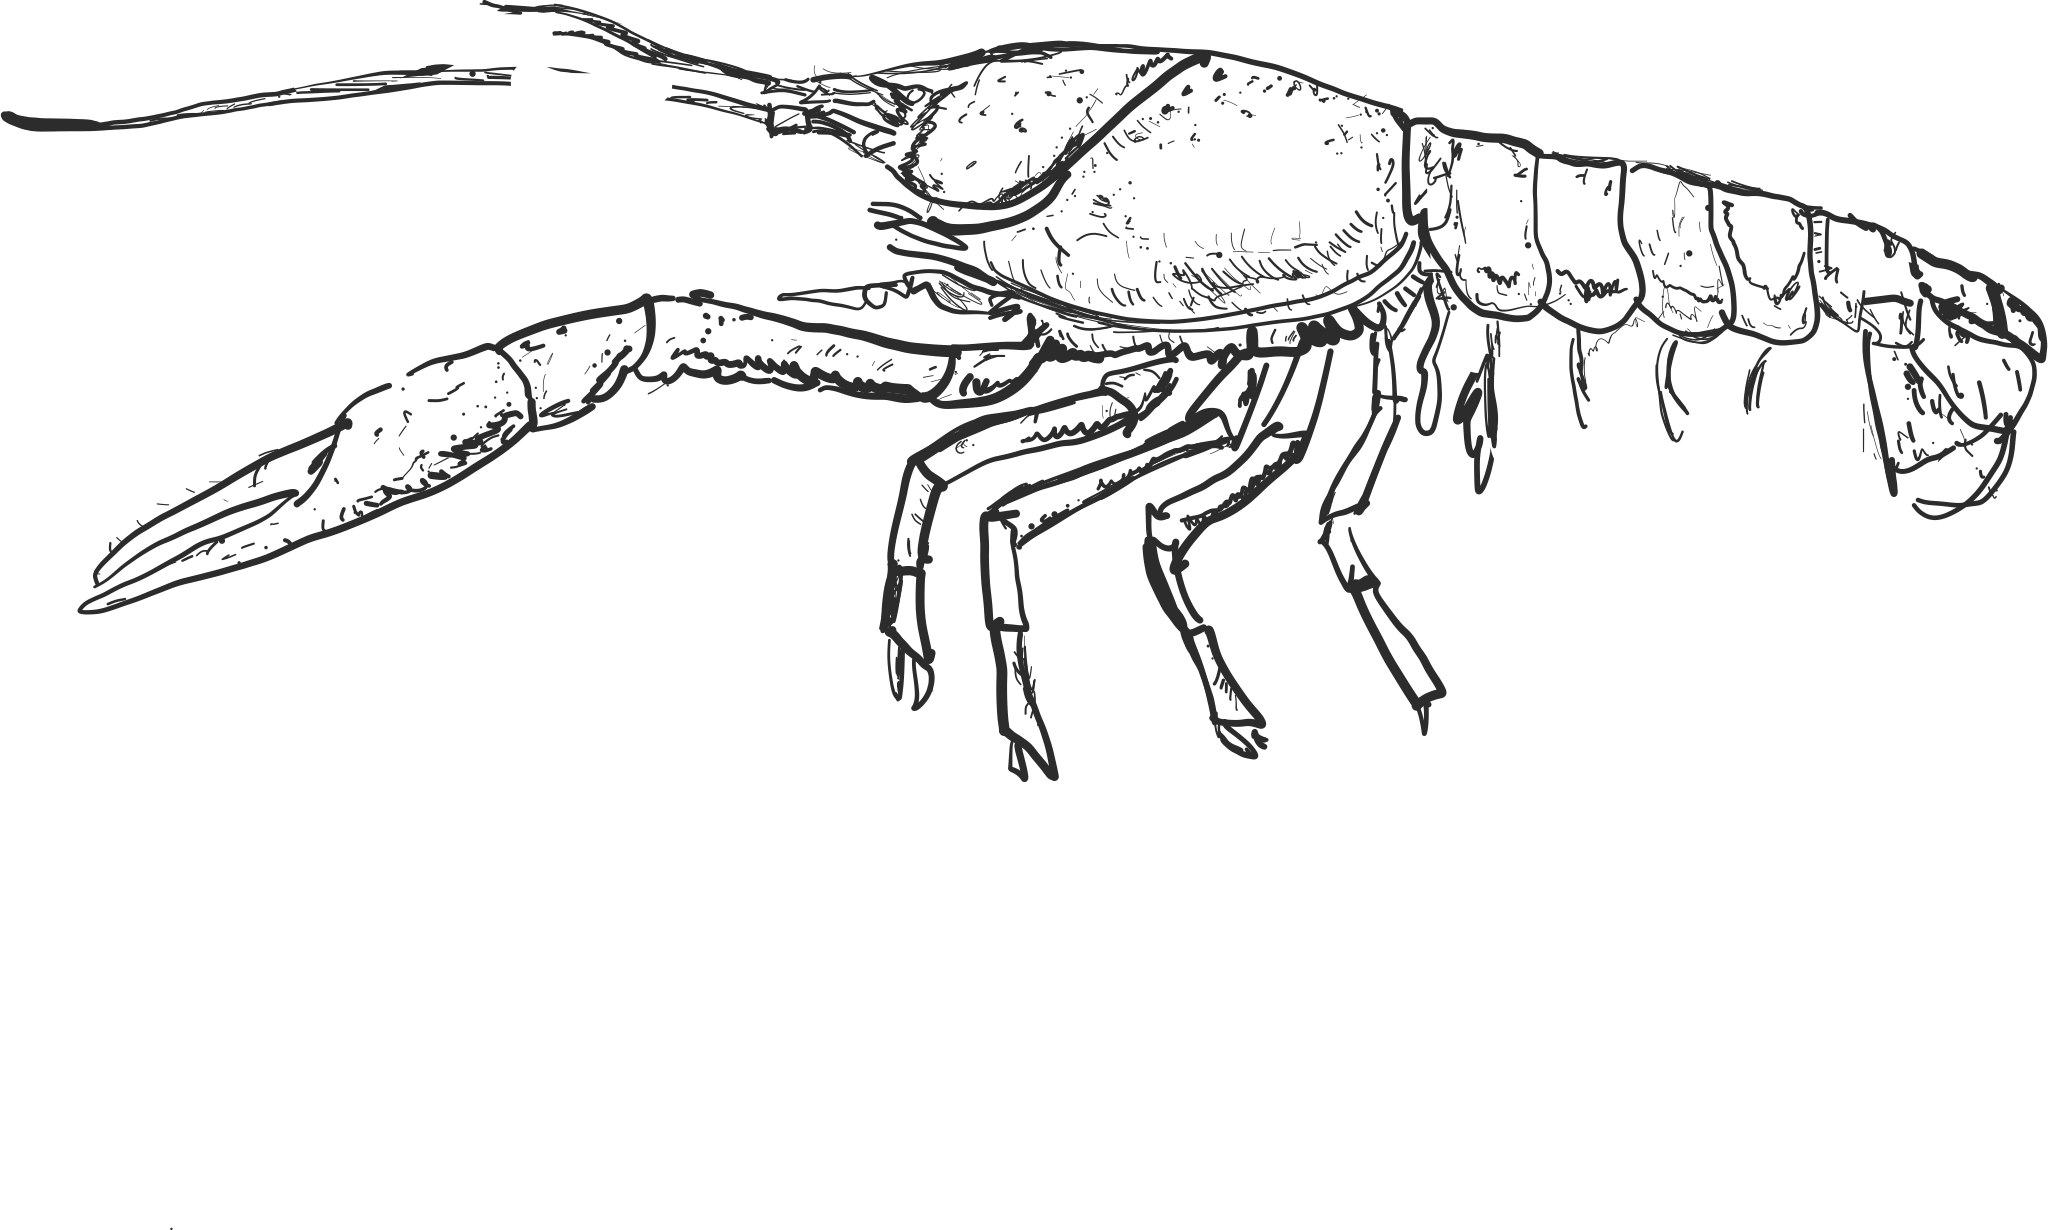
\includegraphics[width=0.7\linewidth]{./figures/nematoda/crayfish}

}

\caption{Crayfish}\label{fig:crayfish}
\end{figure}

\begin{figure}

{\centering 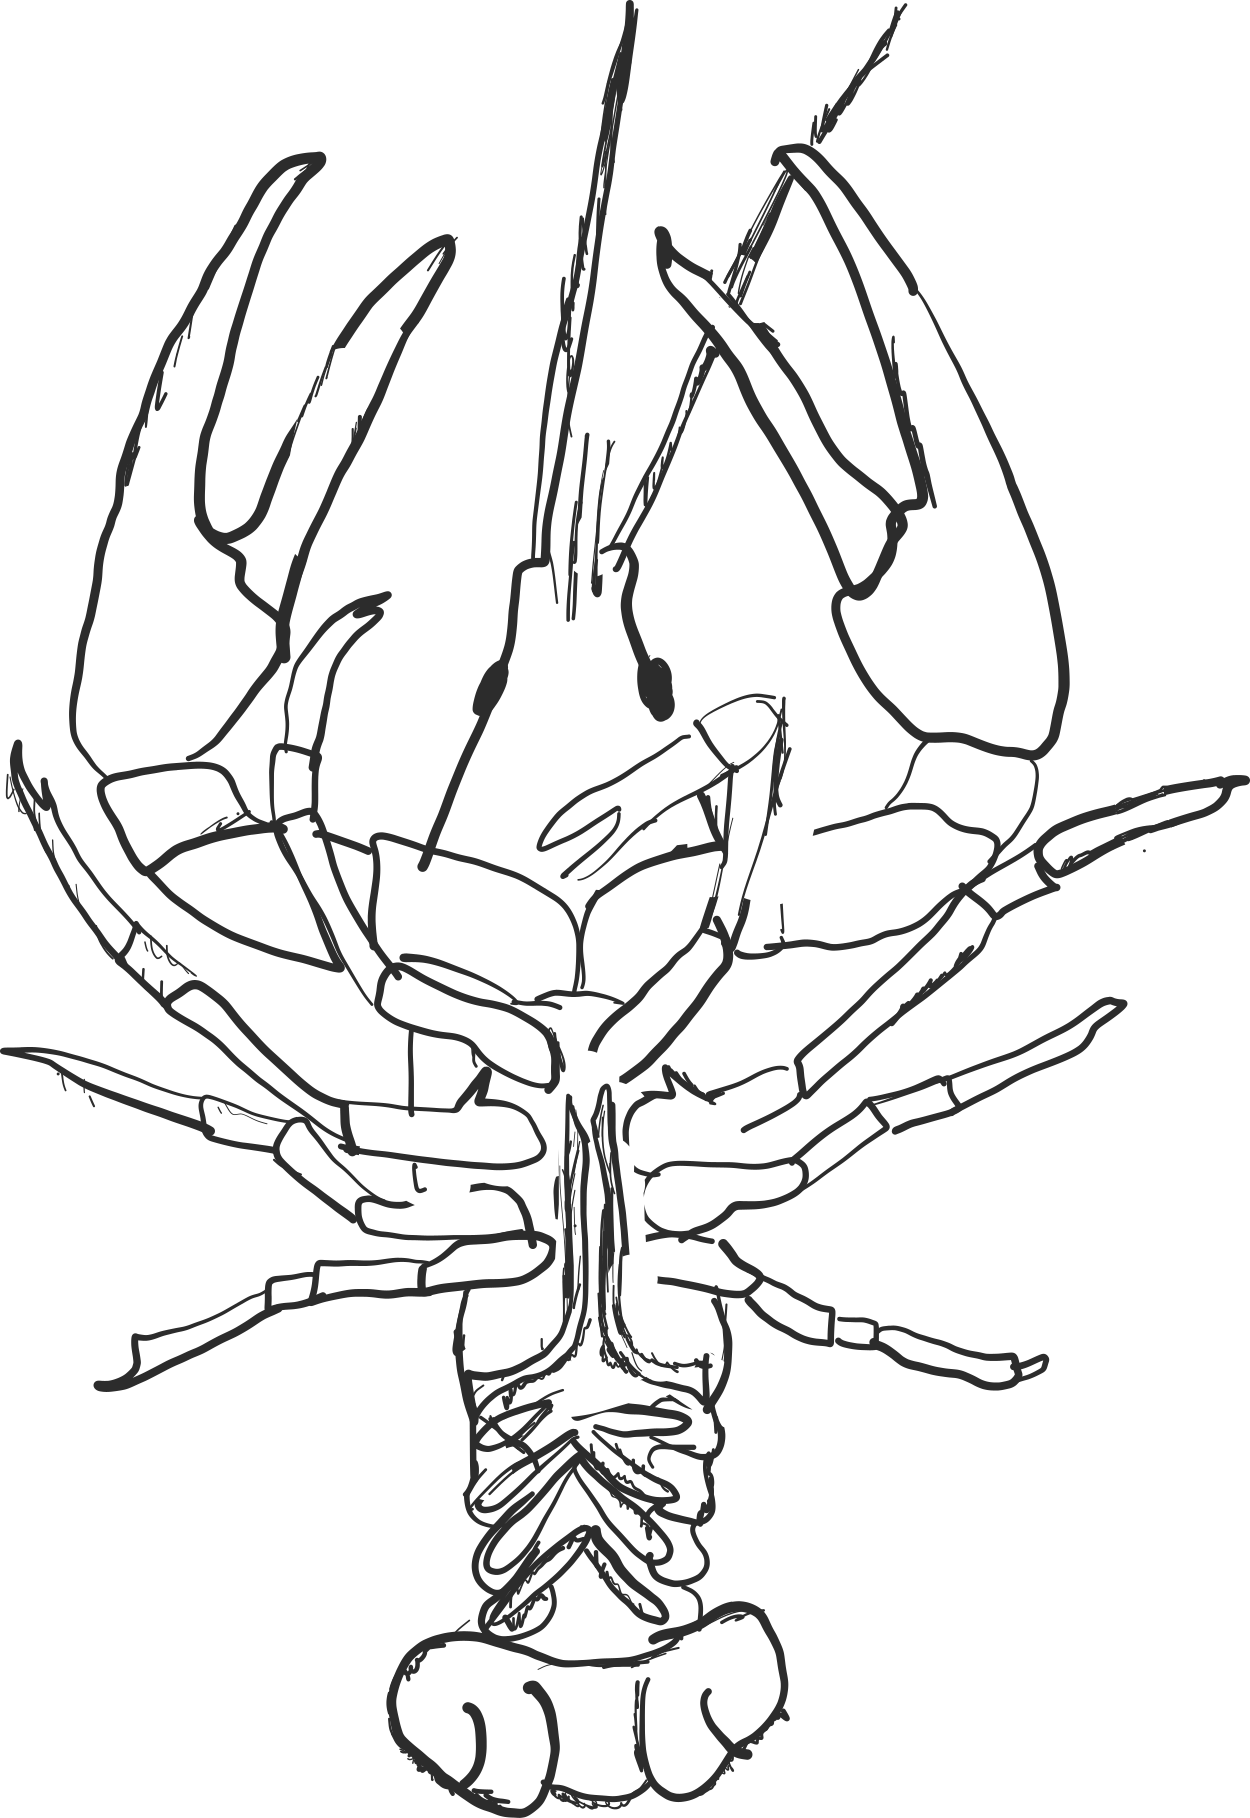
\includegraphics[width=0.7\linewidth]{./figures/nematoda/male_crayfish}

}

\caption{Ventral view of a male crayfish. Notice the gonapods and hooks.}\label{fig:malecray}
\end{figure}

\begin{figure}

{\centering \includegraphics[width=0.7\linewidth]{./figures/nematoda/female_crayfish}

}

\caption{Ventral view of a female crayfish. Notice the central opening to the seminal receptacle.}\label{fig:femalecray}
\end{figure}

\begin{figure}

{\centering \includegraphics[width=0.7\linewidth]{./figures/nematoda/crayfish_dorsal}

}

\caption{Dorsal view of the crayfish. Cut along the dotted lines.}\label{fig:dorsal}
\end{figure}

\begin{figure}

{\centering 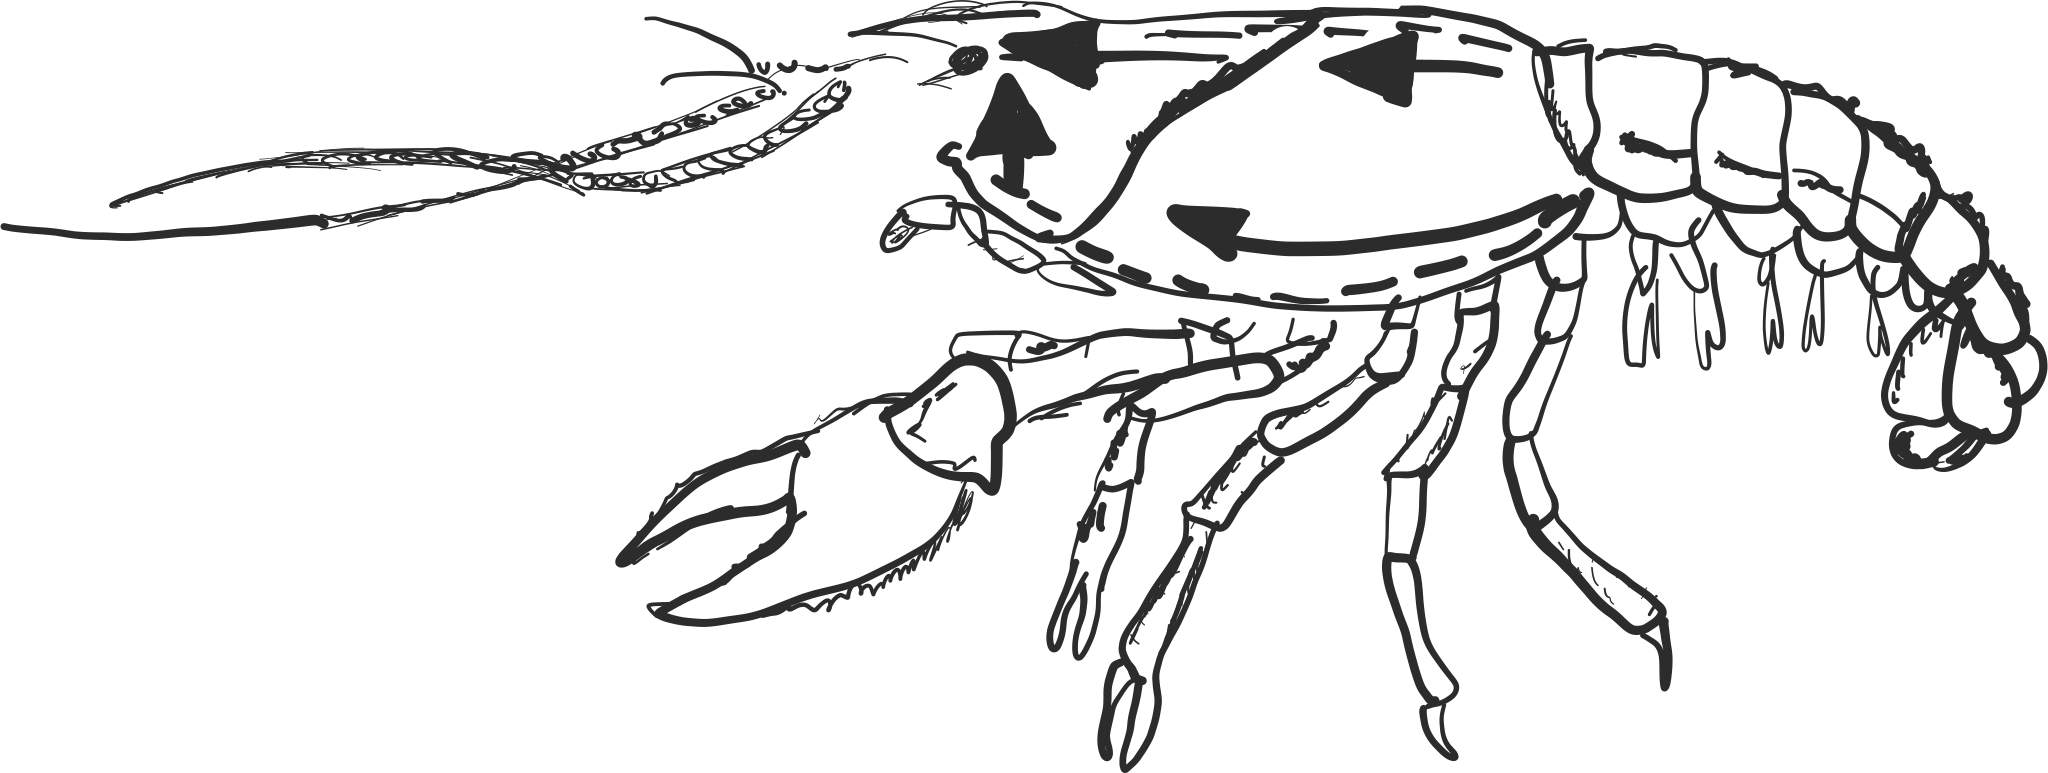
\includegraphics[width=0.7\linewidth]{./figures/nematoda/crayfish_lateral}

}

\caption{Lateral view of the crayfish. Cut along the dotted lines.}\label{fig:lateral}
\end{figure}

\begin{figure}

{\centering \includegraphics[width=0.7\linewidth]{./figures/nematoda/crayfish_brain_and_stomach} 

}

\caption{The crayfish brain and cardiac and pyloric stomach.}\label{fig:brain}
\end{figure}

\begin{figure}

{\centering \includegraphics[width=0.7\linewidth]{./figures/nematoda/crayfish_heart} 

}

\caption{The crayfish heart. Notice the holes in the lateral walls.}\label{fig:heart}
\end{figure}

\begin{figure}

{\centering \includegraphics[width=0.7\linewidth]{./figures/nematoda/crayfish_teeth} 

}

\caption{Teeth in the stomach of the crayfish.}\label{fig:teeth}
\end{figure}

\begin{figure}

{\centering \includegraphics[width=0.7\linewidth]{./figures/nematoda/crayfish_green_gland} 

}

\caption{The green glands (also called maxillary or antennal glands) of the crayfish.}\label{fig:gland}
\end{figure}

\section{Cleaning up}\label{cleaning-up-2}

\begin{enumerate}
\def\labelenumi{\arabic{enumi}.}
\tightlist
\item
  Dispose of the remains of the crayfish in the red biohazard bins.
\item
  Clean the dissection tray and instruments and return them to the place
  where you picked them up.
\item
  Clean table tops with red bottled sanitizer.
\item
  Wash your hands.
\end{enumerate}

\section{View Living Organisms}\label{view-living-organisms-4}

\begin{enumerate}
\def\labelenumi{\arabic{enumi}.}
\tightlist
\item
  Vinegar eels
\item
  Mixed crustaceans

  \begin{itemize}
  \tightlist
  \item
    Look for isopods (sow bugs), amphipods, copepods, water fleas
    (Daphnia), ostracods, and fairy shrimp.
  \end{itemize}
\end{enumerate}

\section{Review Questions}\label{review-questions-5}

\begin{enumerate}
\def\labelenumi{\arabic{enumi}.}
\tightlist
\item
  What are nematodes?
\item
  What are arthropods?
\item
  What is an exoskeleton?
\item
  What are crustaceans?
\end{enumerate}
